\documentclass[tikz,border=10pt]{standalone}
\usepackage{tikz}
\usepackage{siunitx} % optional, if you want nice units

\usetikzlibrary{backgrounds}

\usetikzlibrary{arrows.meta,calc,patterns}

\begin{document}
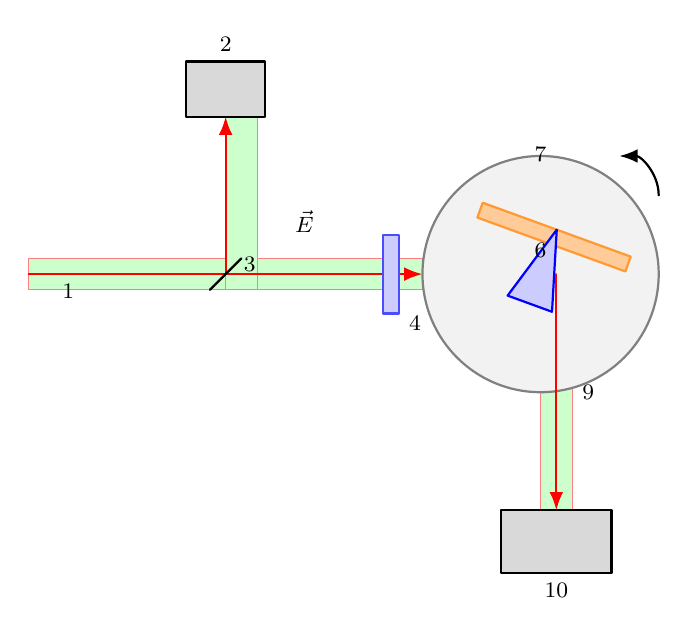
\begin{tikzpicture}[
    font=\footnotesize,
    line cap=round, 
    line join=round,
    >=Latex,                % arrow tip style
    thick
]

%-----------------------
% 1) MAIN HORIZONTAL BEAM
%-----------------------
% Draw a broad "beam" using a colored rectangle to mimic the pink path
\begin{scope}[on background layer] % so the beam is drawn "behind" other elements
  \path[fill=green!20, draw=red!50] (-0.5,-0.2) rectangle (4.5,0.2);
\end{scope}

% Arrow along the beam
\draw[->,red] (-0.5,0) -- (4.5,0);

\node[below] at (0.0,0) {1}; 

%-----------------------
% 2) CAMERA (TOP)J
%-----------------------
% Part of the beam is reflected upward
% For the reflection path, we draw a small rectangle as the "beam"
\begin{scope}[on background layer]
  \path[fill=green!20, draw=red!50] (2,-0.2) -- (2,2) -- (2.4,2) -- (2.4,-0.2) -- cycle;
\end{scope}
\draw[->,red] (2,0) -- (2,2);

% A small box representing the camera
\draw[fill=gray!30] (1.5,2) rectangle (2.5,2.7);
\node[above] at (2,2.7) {2};

%-----------------------
% 3) BEAMSPLITTER
%-----------------------
% A diagonal line to represent the partially reflecting mirror
\draw[thick] (1.8,-0.2) -- (2.2,0.2);
\node[above right] at (2.1,-0.1) {3};

%-----------------------
% 4) FILTER/SHUTTER
%-----------------------
\draw[fill=blue!20,draw=blue!70] (4,0.5) rectangle (4.2,-0.5);
\node[below right] at (4.2,-0.4) {4};

% An arrow indicating the polarization E (just a decorative label)
\node[above] at (3,0.4) {$\vec{E}$};

%-----------------------
% 5–7) ROTATION STAGE, SAMPLE, ETC.
%-----------------------
% Draw a circle for the stage
\draw[fill=gray!10,draw=gray] (6,0) circle (1.5);
\node at (6,0) {5};

% A rectangular “holder” at an angle for the sample
\begin{scope}[rotate around={-20:(6,0)}] % rotate about center (6,0)
  \draw[fill=orange!40,draw=orange!80] (6-1.0,0.4) rectangle (6+1.0,0.6);
\end{scope}
\node[above] at (6,1.3) {7};

% A triangular prism inside to represent sample/wedge
\begin{scope}[rotate around={-20:(6,0)}]
  \path[fill=blue!20,draw=blue] (5.7,-0.4) -- (6.0,0.6) -- (6.3,-0.4) -- cycle;
\end{scope}
\node at (6,0.3) {6};

% Optional arrow to illustrate rotation
\draw[->,thick] (7.5,1) arc (0:90:0.5);

%-----------------------
% 8–10) BEAM EXIT & DETECTOR
%-----------------------
% Another beam going downward from the wedge
\begin{scope}[on background layer]
  \path[fill=green!20, draw=red!50] (6.0,-0.2) rectangle (6.4,-3.0);
\end{scope}
\draw[->,red] (6.2,0) -- (6.2,-3);

\node[right] at (6.4,-1.5) {9};

% A detector box at the bottom
\draw[fill=gray!30] (5.5,-3) rectangle (6.9,-3.8);
\node[below] at (6.2,-3.8) {10};

\end{tikzpicture}
\end{document}
